\chapter{Implementação e resultados}
\label{cap:implementacaoresultados}

Neste capítulo será apresetado o projeto de implementação, detalhado a implementação com a configuração do \ac{OS}, do ambiente virtualizado e 
das ferramentas que irão compôr o \textit{cluster} de alta disponibilidade. Posteriormente, será apresentada a metodologia de testes e 
apresentado os resultados das medições para validação da alta disponibilidade.

\section{Implementação}
\label{section:implementacao}

O ambiente foi configurado na forma de um \textit{cluster}, o qual é composto por dois servidores com requisitos de configuração 
de 12 \textit{cores} de processamento, 14 GB de memória \ac{RAM} e 180 GB de disco rígido.
%real = 11 \textit{cores} de processamento, 12 GB de memória \ac{RAM} e 156 GB de disco rígido
Essa configuração inclui 2 GB de memória \ac{RAM} e 24 GB de disco para cada sistema operacional hóspede. Além disso, optou-se por utilizar o 
mesmo sistema operacional e o mesmo hipervisor que são adotados atualmente na empresa, o sistema \textit{Ubuntu 14.04 \ac{LTS}} e o \ac{KVM} 
\cite{kvm}, respectivamente. O detalhamento da instalação e configuração encontra-se no APENDICE A 1 E 4 ??.

A estrutura física adotada está representada na Figura \ref{fig:projeto_fisico}. Pode-se observar os dois servidores ligados a um 
\textit{switch} através de dois cabos UTP, ou seja, cada servidor encontra-se conectado ao \textit{switch} através de dois cabos, de forma a 
implementar uma redundância do cabeamento.

\begin{figure}[h!]
 \centering
 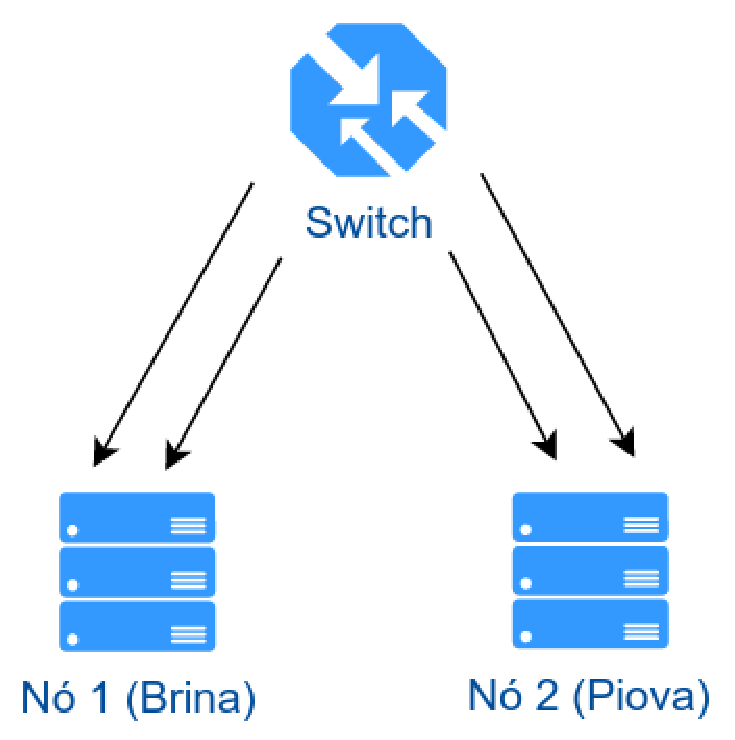
\includegraphics[width=180px]{img/projeto_fisico.eps}
 \caption{Estrutura física.}
 \label{fig:projeto_fisico}
\end{figure}

Para a configuração de rede manteve-se o \textit{link aggregation} e utilizou-se uma \textit{bridge} para incluir as máquinas virtuais à rede.
Os detalhes da configuração estão localizados no APENDICE A 2 ??.

Na Figura \ref{fig:servidores_brina_piova} tem-se a imagem dos servidores, o primeiro é o \textit{Brina} (\textit{Dell PowerEdge 2950}), 
e o segundo servidor é o \textit{Piova} (\textit{Dell PowerEdge R410}).

\begin{figure}[h!]
 \centering
 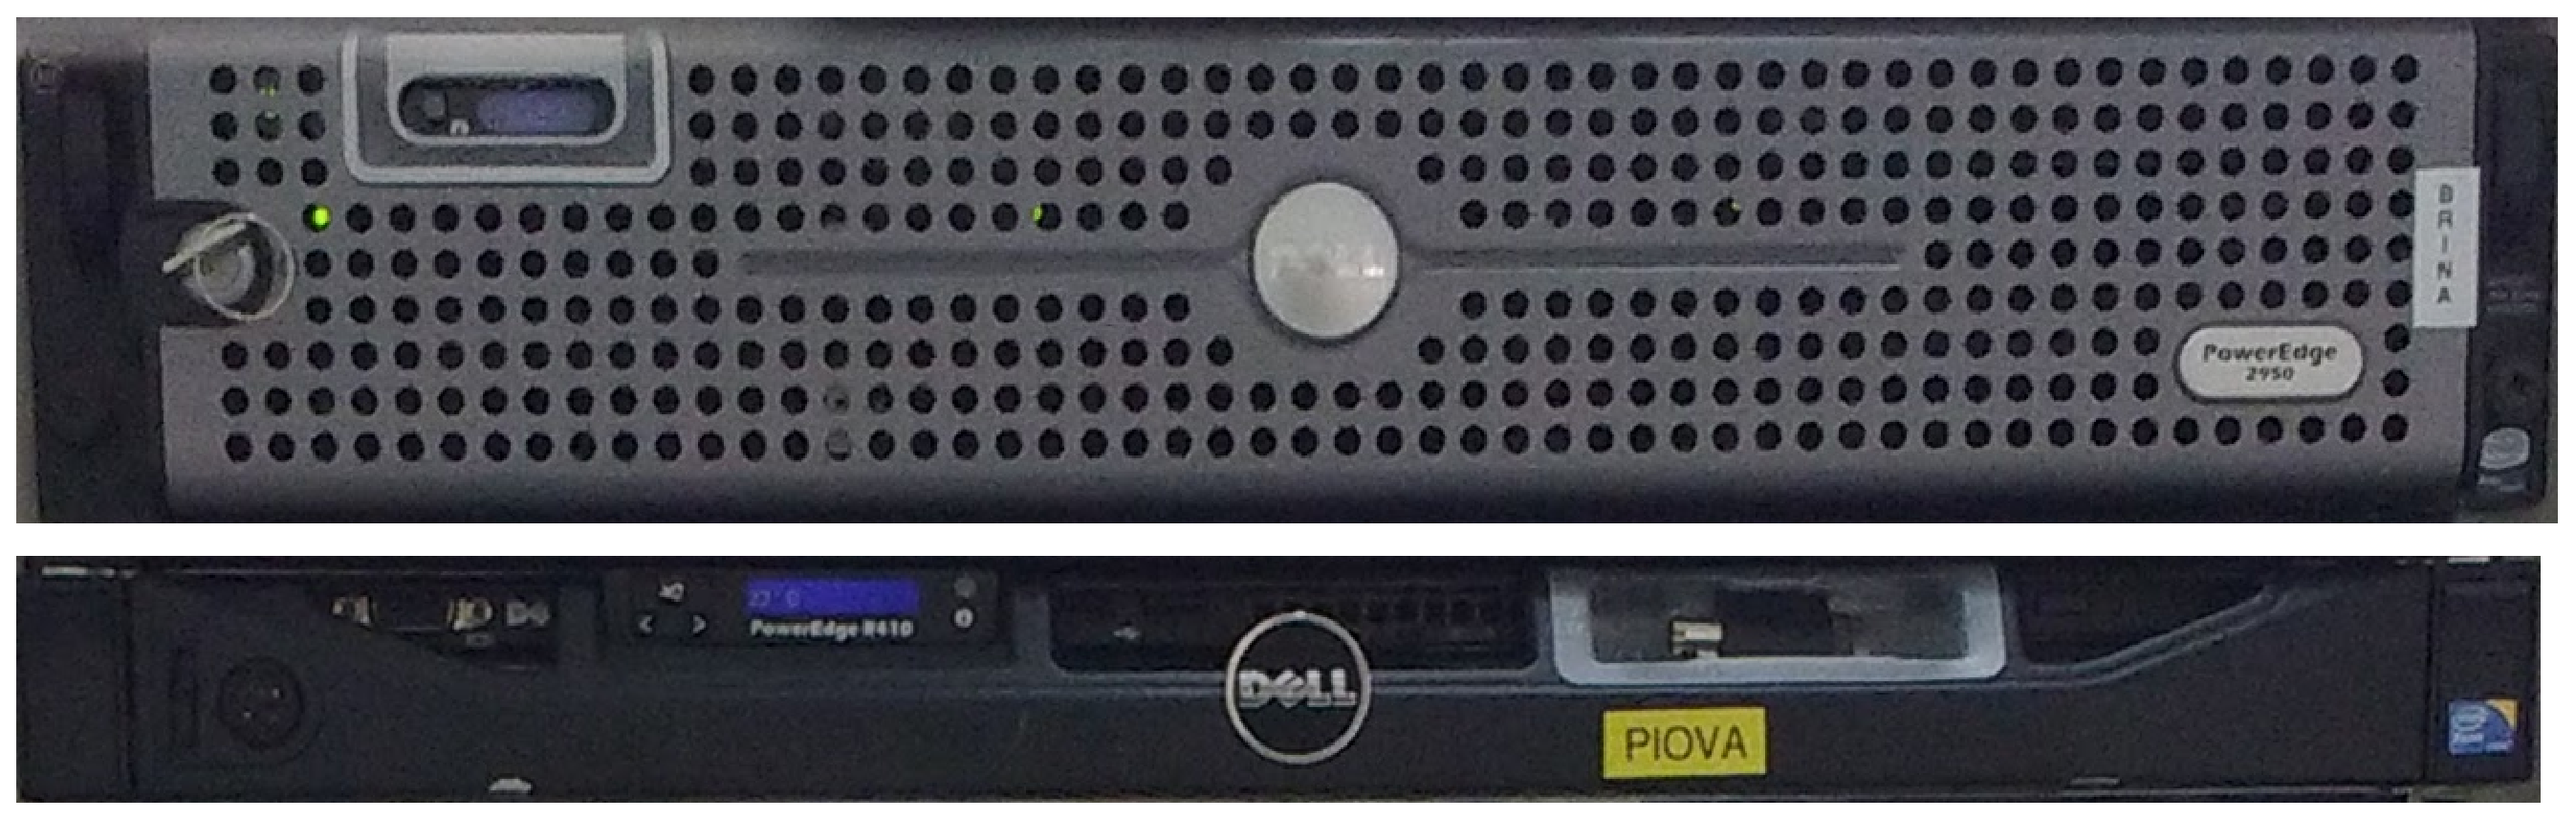
\includegraphics[width=300px]{img/servidores_brina_piova.eps}
 \caption{Servidores.}
 \label{fig:servidores_brina_piova}
\end{figure}

A estrutura lógica dos servidores juntamente com as máquinas virtuais e seus respectivos serviços são apresentados na Figura 
\ref{fig:projeto_estrutura}. Para a replicação de dados foi utilizado o \textit{software} \ac{DRBD}, que foi configurado no modo 
\textit{dual-master} onde os dois nós são configurados como primários. Para tal configuração é necessário utilizar um sistema de arquivos 
distribuídos que faz o gerenciamento do acesso aos dados, o \textit{software} adotado foi o \ac{OCFS2}. 
Os detalhes da instalação e da configuração de disco, \ac{DRBD} e sistema de arquivos estão detalhadas no APENDICE A 3 ??. 
O \textit{software} \textit{Pacemaker} faz o gerenciamento do \textit{cluster}, sendo responsável pela gerência, monitoramento e migração das 
\acp{VM} entre os nós.

\begin{figure}[h!]
 \centering
 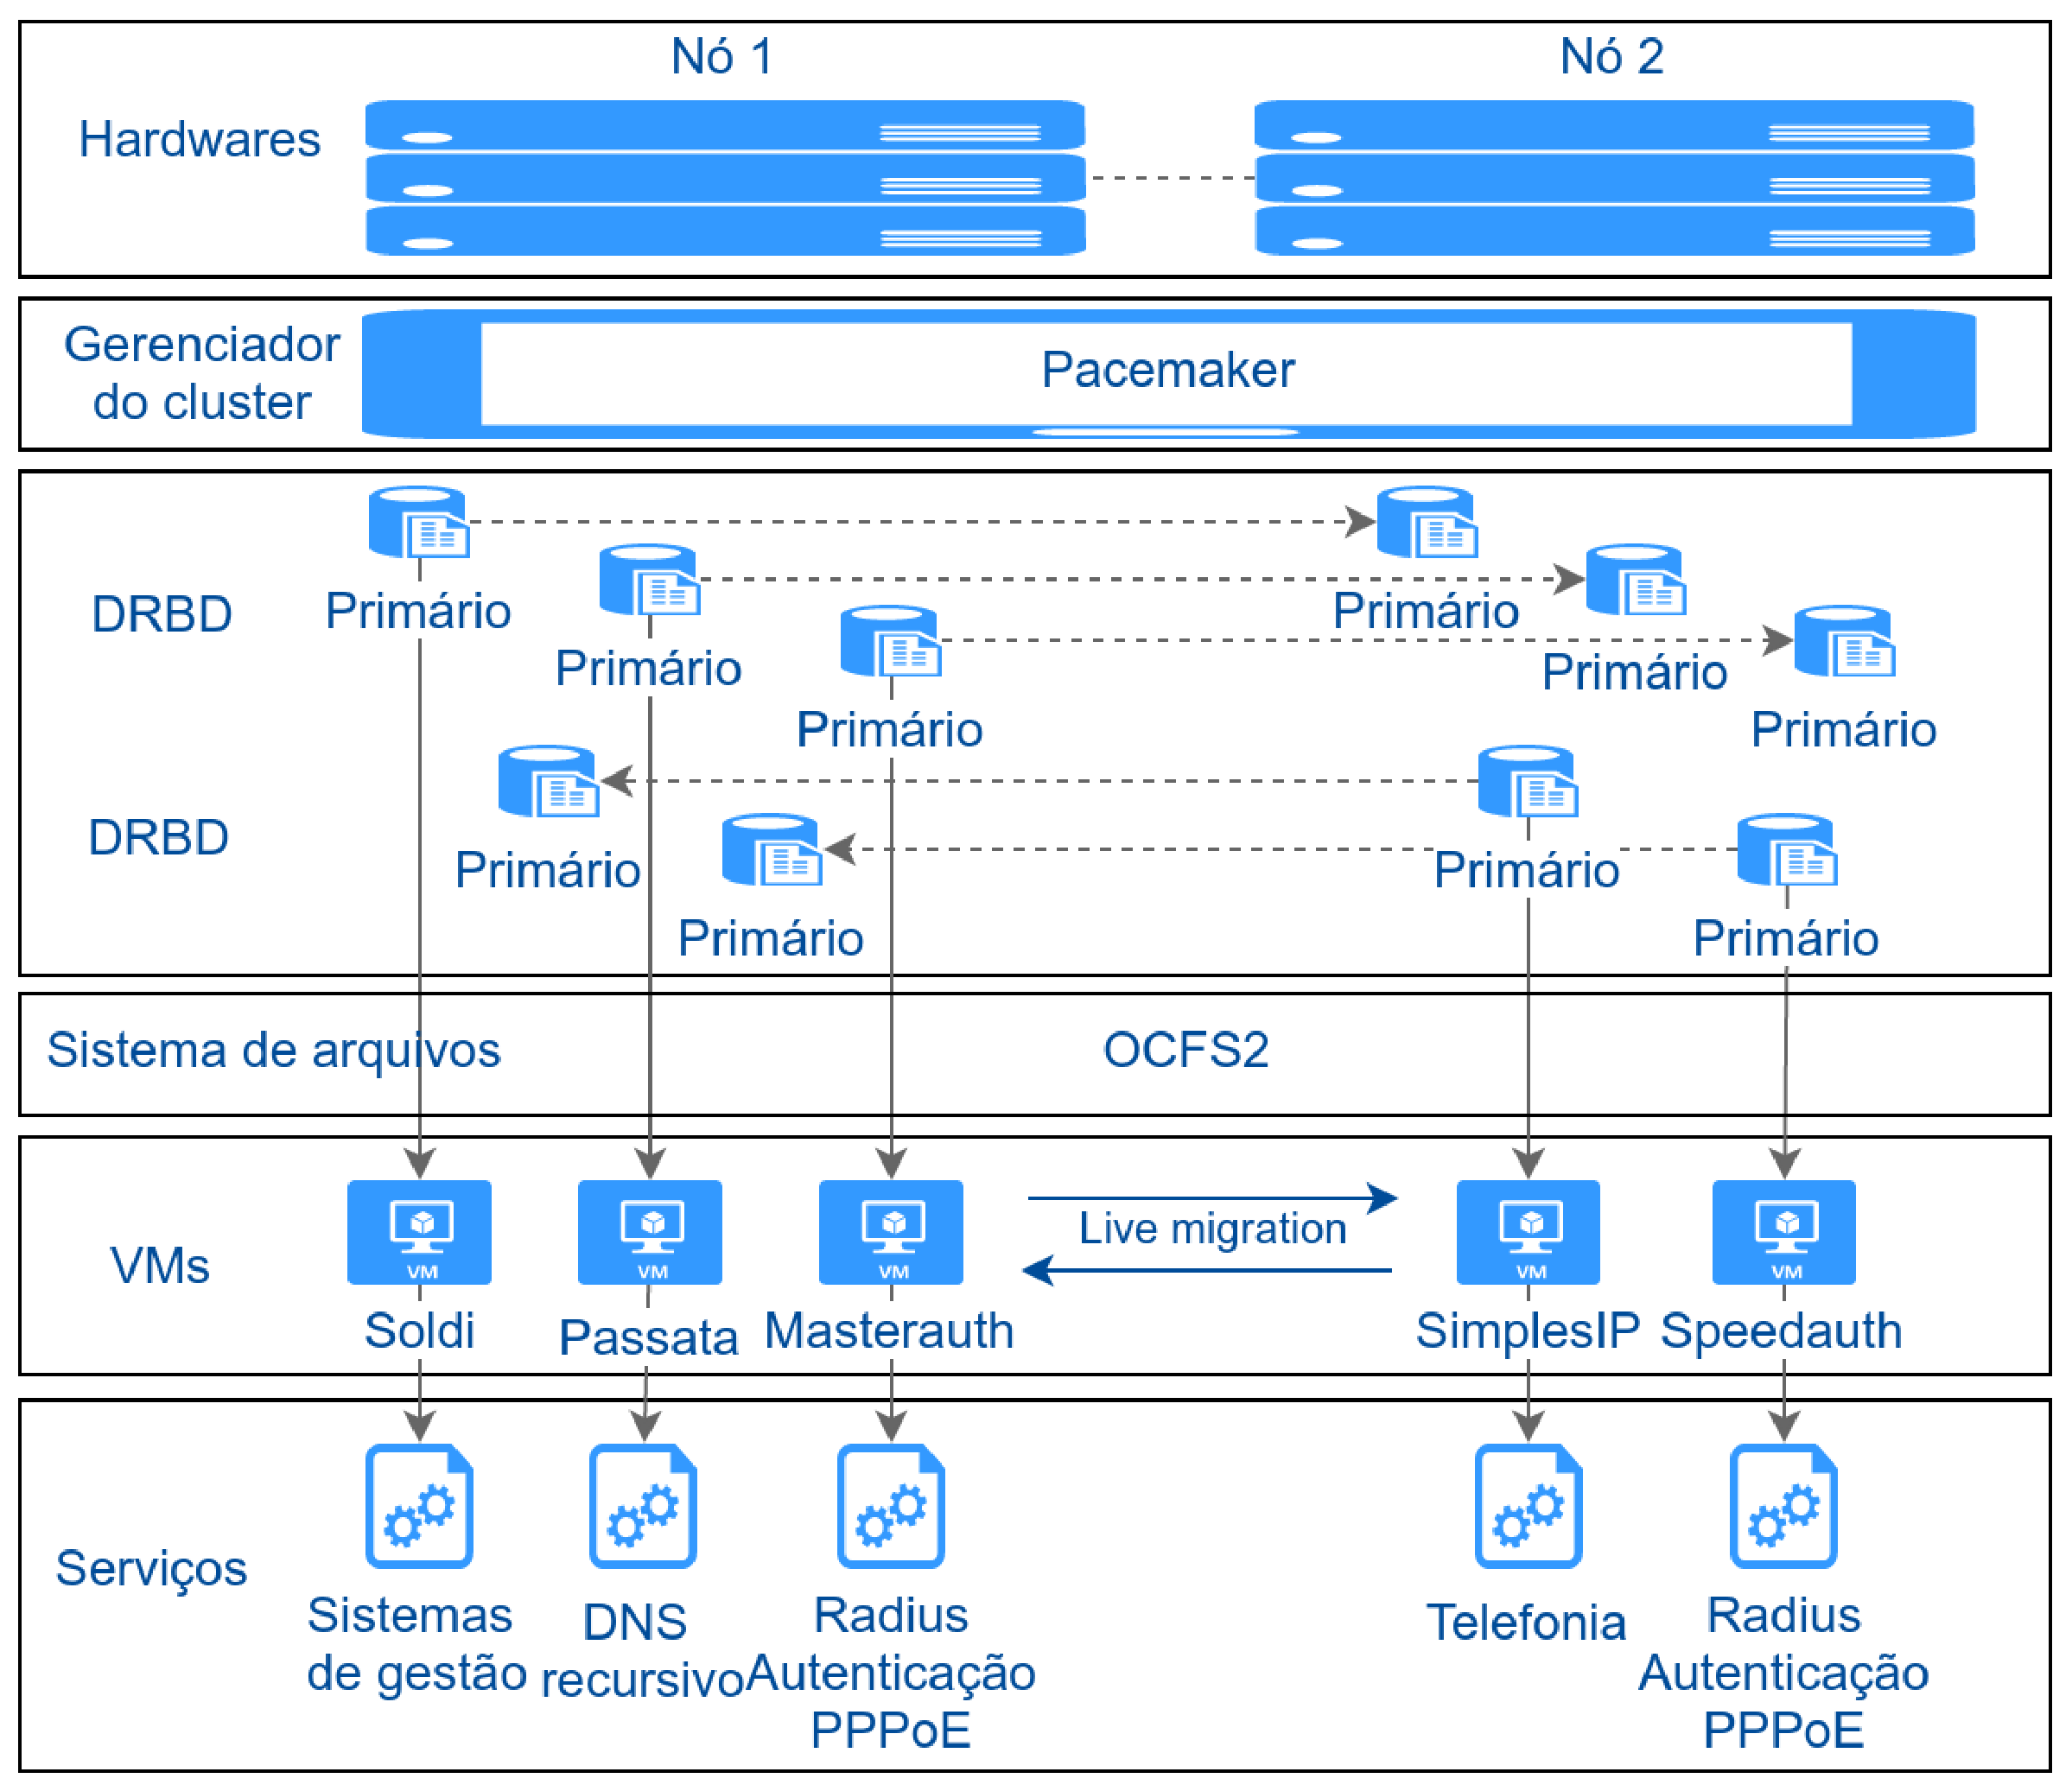
\includegraphics[width=350px]{img/projeto_estrutura.eps}
 \caption{Estrutura do \textit{cluster}.}
 \label{fig:projeto_estrutura}
\end{figure}

%drbd
% O \ac{DRBD} será configurado no modo \textit{master-slave}, sendo que para cada disco das máquinas virtuais será criado um dispositivo de 
% replicação \ac{DRBD}. E para utilizar esse dispositivo como disco de uma máquina virtual será criado um volume lógico 
% \ac{LVM}\footnote{LVM é uma ferramenta de código aberto que possibilita a manipulação de discos rígidos, através da criação de grupos de volumes 
% e volumes lógicos para \textit{Linux}.} \cite{lvm}. 

Deste modo, tem-se o ambiente pronto para a criação das \acp{VM}, sendo assim criou-se uma instância para cada servidor virtual. 
Como pode ser observado no Figura \ref{fig:projeto_estrutura}, criou-se três instâncias no Nó 1 e duas instâncias no outro Nó 2. De fato, o 
primeiro possui as instâncias dos servidores \textit{Soldi}, \textit{Passata} e \textit{Masterauth}. Já o segundo nó possui as instâncias dos 
servidores \textit{SimplesIP} e \textit{Speedauth}. Desta forma, quando houver uma falha em um nó, as instâncias serão iniciadas no nó disponível.
O detalhamento da configuração do \textit{Pacemaker} estão no APENDICE A 5 ??.


\section{Testes}
\label{section:testes}

objetivo também é compravar que a gerência da manutenção e a gerência de falhas são importantes para um ambiente...

VER??
Validação, metodologia de testes:
-Desligamento físico (simulação falha de hardware ou eletrica): 4 vezes para medir tempo de downtime dos servicos e dos nodes (servico nao critico)
-Desligamento por software (reboot manual): 4 vezes para medir tempo de downtime dos servicos e dos nodes (servico nao critico)
-Agendamento de manutenção (reboot para atualização de software): 2 semanas ou mais, 1 manutenção por semana, com live migration, reboot e 
atualizacao de kernel dos nodes
-Medicao da disponibilidade dos serviços críticos por 1 mes (setembro)

Medição através do Nagios, que utiliza ping para calcular o tempo de downtime
Tabela com perda de pacotes, latencia, tempo de indisponibilidade



APENDICE
VERBOS PRESENTE?

\section{Configuração do \ac{OS}}

Foi feita a instalação do sistema operacional \textit{Ubuntu 14.04 \ac{LTS}} nos dois servidores. A configuração feita foi a básica do sistema,
com nome do servidor, configuração de rede, localização e instalação do servidor \ac{SSH}.
Além disso, é feito as configurações padrões adotadas pela empresa, como por exemplo, ferramentas de monitoramento, atualização automática
e \textit{firewall}.

\section{Configuração de rede}

Uma forma de incluir as máquinas virtuais a uma rede é através da criação de uma \textit{bridge}. A instalação é feita através do comando:
\begin{lstlisting}[language=bash]
  $ apt-get install bridge-utils
\end{lstlisting}

Além disso, é necessário instalar e configurar o \textit{link aggregation}, o \textit{Ubuntu} usa o padrão \textit{IEEE 802.3ad}. A configuração 
é feita no servidor e no \textit{switch}. Abaixo tem-se os comandos para instalação do \textit{link aggregation}, o primeiro comando faz a 
instalação e o segundo comando carrega o modulo \textit{bonding} no \textit{kernel}:
\begin{lstlisting}[language=bash]
 $ apt-get install ifenslave-2.6
 $ sh -c 'grep -q bonding /etc/modules || echo bonding >> /etc/modules'
\end{lstlisting}

Para a configuração do \textit{link aggregation} deve-se criar uma interface \textit{bond} e nela inclui-se as duas interfaces físicas.
Abaixo tem-se a configuração de rede, que inclui o \textit{link aggregation} e a \textit{bridge}, esta configuração deve ser colocada no 
arquivo \textit{/etc/network/interfaces} em cada nó:
\begin{lstlisting}
auto eth0
iface eth0 inet manual
bond-master bond0

auto eth1
iface eth1 inet manual
bond-master bond0

auto bond0
iface bond0 inet manual
       bond-mode 4
       bond-slaves eth0 eth1
       bond-lacp-rate 1
       bond-miimon 100
       bond-xmit_hash_policy layer3+4

auto br0
iface br0 inet static
       address x.x.x.x
       netmask 255.255.255.0
       network x.x.x.0
       broadcast x.x.x.255
       gateway x.x.x.x
       dns-nameservers 8.8.8.8 8.8.4.4
       
       bridge_ports bond0
       bridge_stp off
       bridge_maxwait 0
\end{lstlisting}

Também é necessário configurar algumas \textit{vlans} para algumas máquinas virtuais. Os comandos a seguir fazem a instalação e carregam
o modulo do \textit{kernel} necessário para gerenciar \textit{vlans}:
\begin{lstlisting}[language=bash]
 $ apt-get install vlan
 $ sudo  sh -c 'grep -q 8021q /etc/modules || echo 8021q >> /etc/modules'
 $ sudo modprobe 8021q
\end{lstlisting}

\section{Configuração de disco}

Os discos que são replicados podem ser utilizados diretamente no \ac{DRBD} (por exemplo \textit{/dev/sda2}) ou configurados com \ac{LVM}. Adotou-se
a configuração utilizando \ac{LVM} pois torna-se mais fácil a manipulação dos discos. O comando abaixo faz a criação de um volume lógico chamado 
\textit{lvdrbd} com tamanho de 500 GB, este volume pertence ao grupo de volumes \textit{vg0}.
\begin{lstlisting}[language=bash]
 $ lvcreate -n lvdrbd vg0 -L 500G
\end{lstlisting}

\subsection{DRBD}

Para a instalação do \textit{software} de replicação de dados é necessário instalar os dois pacotes, que estão listados abaixo:
\begin{lstlisting}[language=bash]
 $ apt-get install drbd8-utils drbdlinks
\end{lstlisting}

É necessário alterar a configuração global do \ac{DRBD} que está localizada em \textit{/etc/drbd.d/global\_common.conf}:
\begin{lstlisting}
global {
        usage-count yes;
        minor-count 16;
}
\end{lstlisting}

Posteriormente, deve-se criar um recurso que definirá os dispositivos de disco, os endereços \ac{IP} e portas dos servidores.
Deve-se criar o arquivo \textit{/etc/drbd.d/vms.res}, o qual armazena essa configuração:
\begin{lstlisting}
 resource vms {
    meta-disk internal;
    device /dev/drbd0;
    protocol C;
    disk {
        fencing resource-only;
        resync-rate 50M;
    }
    handlers {
        fence-peer "/usr/lib/drbd/crm-fence-peer.sh";
        after-resync-target "/usr/lib/drbd/crm-unfence-peer.sh";
    }
    net {
        allow-two-primaries;
    }
    startup {
        become-primary-on both;
    }
    on brina {
        address x.x.x.x:7791;
        disk /dev/vg0/lvdrbd;
    }
    on piova {
        address y.y.y.y:7791;
        disk /dev/vg0/lvdrbd;
    }
}
\end{lstlisting}

Para o funcionamento correto dessa ferramenta, o nome dos servidores (localizado em \textit{/etc/hostname}) deve ser exatamente igual a opção
\textit{on} da configuração do recurso.

Após ter sido feita a configuração do \ac{DRBD}, deve-se reiniciar o serviço para aplicá-la:
\begin{lstlisting}[language=bash]
 $ service drbd restart 
\end{lstlisting}

Os comandos abaixo, inicializam os discos do \ac{DRBD}, conectam ao outro nó e elegem um nó como primário, respectivamente, para iniciar o 
sincronismo dos dados:
\begin{lstlisting}[language=bash]
 $ drbdadm create-md vms
 $ drbdadm up vms
 $ drbdadm -- --overwrite-data-of-peer primary vms
\end{lstlisting}

E por fim pode-se verificar o estado dos recursos do \ac{DRBD} através do comando:
\begin{lstlisting}[language=bash]
 $ service drbd status
\end{lstlisting}

\subsection{OCFS2}

O \ac{OCFS2} é um sistema de arquivos para \textit{cluster}, ele faz o gerencimento do acesso aos dados (\textit{locks}) que é necessário para o 
funcionamento do \textit{Pacemaker}. Para seu funcionamento é necessário a instalação de um pacote:
\begin{lstlisting}[language=bash]
 $ apt-get install ocfs2-tools
\end{lstlisting}

É preciso fazer duas configurações, a primeira para criar o \textit{cluster}, localizada no arquivo \textit{/etc/ocfs2/cluster.conf}:
\begin{lstlisting}
node:
        ip_port = 7777
        ip_address = x.x.x.x
        number = 0
        name = brina
        cluster = clusterocfs
node:
        ip_port = 7777
        ip_address = y.y.y.y
        number = 1
        name = piova
        cluster = clusterocfs
cluster:
        node_count = 2
        name = clusterocfs
\end{lstlisting}

A segunda configuração é feita no arquivo \textit{/etc/default/o2cb}, ela faz o carregamento do \textit{driver} no \textit{boot} e a definição 
do nome do cluster para inicialização:
\begin{lstlisting}
O2CB_ENABLED=true
O2CB_BOOTCLUSTER=clusterocfs
\end{lstlisting}

Para aplicar as configurações deve-se reiniciar o serviço:
\begin{lstlisting}[language=bash]
 $ service ocfs2 restart
\end{lstlisting}

E por fim, deve-se construir o sistema de arquivos no dispositivo criado pelo \ac{DRBD}, através do comando:
\begin{lstlisting}[language=bash]
 $ mkfs.ocfs2 /dev/drbd/by-res/vms
\end{lstlisting}

%bug ocfs2
Na versão 1.6.4 do pacote \textit{ocfs2-tools} no \textit{Ubuntu 14.04} há um \textit{bug}\footnote{Detalhes do \textit{bug}: 
https://bugs.launchpad.net/ubuntu/+source/ocfs2-tools/+bug/1412438} que impede o \textit{Pacemaker} de montar o sistema de arquivo \ac{OCFS2}. 
Para corrigi-lo deve aplicar o \textit{patch} abaixo no arquivo \textit{/usr/lib/ocf/resource.d/heartbeat/Filesystem}:
\begin{lstlisting}
--- Filesystem 2013-12-16 07:41:25.000000000 +0000
+++ Filesystem.new 2015-01-19 19:01:30.181772112 +0000
@@ -338,7 +338,7 @@ ocfs2_init()
  # not need this:
  OCFS2_SLES10=""
- if [ "X$HA_cluster_type" = "Xcman" ]; then
+ if [ "X$HA_cluster_type" = "Xcorosync" ]; then
      return
  elif [ "X$HA_cluster_type" != "Xopenais" ]; then
   if grep -q "SUSE Linux Enterprise Server 10" /etc/SuSE-release >/dev/null 2>&1 ; then
\end{lstlisting}

\section{Configuração do ambiente virtualizado}

Como já mencionado anteriormente o hipervisor utilizado pela empresa é o \ac{KVM}. Para a virtualização das máquinas também é utilizado a 
\ac{API} \textit{libvirt}, que faz o gerenciamento da virtualização. O comando abaixo faz a instalação dessas ferramentas:
\begin{lstlisting}[language=bash]
 $ apt-get install qemu-kvm libvirt-bin
\end{lstlisting}

Para incluir as máquinas virtuais é necessário criar um \textit{pool}, onde serão armazenadas suas imagens, os comandos abaixo criam a pasta
e o \textit{pool}:
\begin{lstlisting}[language=bash]
 $ mkdir /var/lib/libvirt/images/ocfs
 $ virsh pool-create-as ocfs --type=dir --target=/var/lib/libvirt/images/ocfs
\end{lstlisting}

Para o funcionamento do \textit{live migration} é preciso fazer a troca das chaves \ac{SSH} do usuário root entre os dois nós.
No nó \textit{Brina}, o primeiro comando cria uma chave \textit{rsa} e o segundo copia a chave para o outro nó:
\begin{lstlisting}[language=bash]
 $ ssh-keygen
 $ ssh-copy-id piova
\end{lstlisting}

E no nó \textit{Piova}, deve-se efetuar o mesmo processo:
\begin{lstlisting}[language=bash]
 $ ssh-keygen
 $ ssh-copy-id brina
\end{lstlisting}

\section{Configuração do cluster}
\label{section:configpacemaker}

\subsection{Pacemaker}

O \textit{Pacemaker} faz monitoramento dos nós do \textit{cluster} e iniciará ou finalizará os serviços (recursos) em caso de falhas de um nó.
No \textit{Pacemaker}, os serviços que são configurados para serem monitorados são chamados de recursos (\textit{resources}).

A primeira etapa é a instalação da ferramenta:
\begin{lstlisting}[language=bash]
 $ apt-get install pacemaker corosync
\end{lstlisting}

Após deve-se configurar o \textit{corosync} para fazer o monitoramento do \textit{cluster}, para isso deve editar o arquivo 
\textit{/etc/corosync/corosync.conf}:
\begin{lstlisting}
totem {
	version: 2
	token: 3000
	token_retransmits_before_loss_const: 10
	join: 60
	consensus: 3600
	vsftype: none
	max_messages: 20
	clear_node_high_bit: yes
 	secauth: on
 	threads: 0
 	rrp_mode: none
        interface {
                # The following values need to be set based on your environment 
                member {
                        memberaddr: x.x.x.x
                }
                member {
                        memberaddr: y.y.y.y
                }
                ringnumber: 0
                bindnetaddr: x.x.x.0
        }
        transport: udpu
}
amf {
	mode: disabled
}
quorum {
        # Quorum for the Pacemaker Cluster Resource Manager
        provider: corosync_votequorum
        expected_votes: 2
	two_node: 1
}
service {
        # Load the Pacemaker Cluster Resource Manager
        ver:       0
        name:      pacemaker
}
aisexec {
        user:   root
        group:  root
}
logging {
        fileline: off
        to_stderr: yes
        to_logfile: no
        to_syslog: yes
        syslog_facility: daemon
        debug: off
        timestamp: on
        logger_subsys {
                subsys: AMF
                debug: off
                tags: enter|leave|trace1|trace2|trace3|trace4|trace6
        }
}
\end{lstlisting}

Ajustar para o \textit{corosync} inicie com o sistema, através da alteração da configuração em \textit{/etc/default/corosync}:
\begin{lstlisting}
 START=yes
\end{lstlisting}

Para a comunicação entre os nós deve-se criar uma chave e copiá-la para o outro nó:
\begin{lstlisting}[language=bash]
 $ corosync-keygen
 $ scp /etc/corosync/authkey piova:/etc/corosync/
\end{lstlisting}

E por fim deve-se reiniciar os serviços:
\begin{lstlisting}[language=bash]
 $ service corosync restart
 $ service pacemaker restart
\end{lstlisting}

Para verificar o estado os \textit{cluster}:
\begin{lstlisting}[language=bash]
 $ crm status
\end{lstlisting}

Após os nós estarem \textit{online} deve-se criar os recursos do \textit{Pacemaker}. Para alterar a configuração pode utilizar os diversos
comandos do \textit{crm}, ou pode-se visualizar e alterar toda configuração através do comando:
\begin{lstlisting}[language=bash]
 $ crm configure edit
\end{lstlisting}

Primeiramente deve-se criar o recurso para o \ac{DRBD}. Esse recurso fará o monitoramento e iniciará os dispositivos nos nós do \ac{DRBD}.
A configuração é:
\begin{lstlisting}
primitive DRBD ocf:linbit:drbd \
        params drbd_resource="vms" \
        op monitor interval="20" role="Master" timeout="240" \
        op monitor interval="30" role="Slave" timeout="240" \
        meta is-managed="true" target-role="Started"
ms MS_DRBD DRBD \
        meta master-max="2" clone-max="2" notify="true" interleave="true" allow-migrate="true" is-managed="true" 
\end{lstlisting}
Onde \textit{primitive} é o recurso \ac{DRBD} configurado anteriormente, e \textit{ms} é a opção que fará o dispositivo se tornar \textit{master}
sendo limitado em 2.

Também será necessário criar um recurso para montar um sistema de arquivos \ac{OCFS2}, configurado da seguinte forma:
\begin{lstlisting}
primitive OCFS_MOUNT ocf:heartbeat:Filesystem \
        params device="/dev/drbd/by-res/vms" directory="/var/lib/libvirt/images/ocfs" fstype="ocfs2"
clone OCFS_MOUNT_CLONE OCFS_MOUNT \
        meta interleave="true" ordered="true" target-role="Started"
colocation COL_DRBD_OCFS inf: OCFS_MOUNT_CLONE MS_DRBD:Master
order ORD_DRBD_OCFS inf: MS_DRBD:promote OCFS_MOUNT_CLONE:start
\end{lstlisting}
Onde \textit{primitive} define qual será o dispositivo e onde será montado, o recurso \textit{clone} permitirá montar o sistema nos dois nós
ao mesmo tempo. Já o \textit{colocation} fará a dependecia entre os recursos do \textit{Pacemaker}, por exemplo, é necessário ter o dispositivo 
\ac{DRBD} como \textit{master} para depois montar o sistema de arquivos. E o recurso \textit{order} identifica a ordem de inicialização dos 
recursos, da equerda para direita.

E por fim, deve-se configurar um recurso para cada máquina virtual no \textit{Pacemaker} para possibilitar que as máquinas virtuais sejam 
iniciadas ou migradas de um nó para outro de forma automática: 
\begin{lstlisting}
primitive VM_1 ocf:heartbeat:VirtualDomain \
        params config="/etc/libvirt/qemu/vm1.xml" hypervisor="qemu:///system" migration_transport="ssh" force_stop="0" \
        op monitor timeout="30" interval="10" depth="0" \
        op start timeout="90" interval="0" \
        op stop timeout="90" interval="0" \
        op migrate_from interval="0" timeout="240" \
        op migrate_to interval="0" timeout="240" \
        meta allow-migrate="true" target-role="Started" is-managed="true" migration-threshold="5"
location cli-prefer-VM_1 VM_1 inf: brina
location backup-VM_1 VM_1 100: piova
colocation COL_VM_1 inf: VM_1 OCFS_MOUNT_CLONE
order ORD_VM_1 inf: OCFS_MOUNT_CLONE:start VM_1:start
\end{lstlisting}

